\documentclass[11pt,border=6pt]{standalone}
\usepackage{fontspec}
\usepackage{tikz}
\usetikzlibrary{positioning,arrows.meta,calc}
\begin{document}
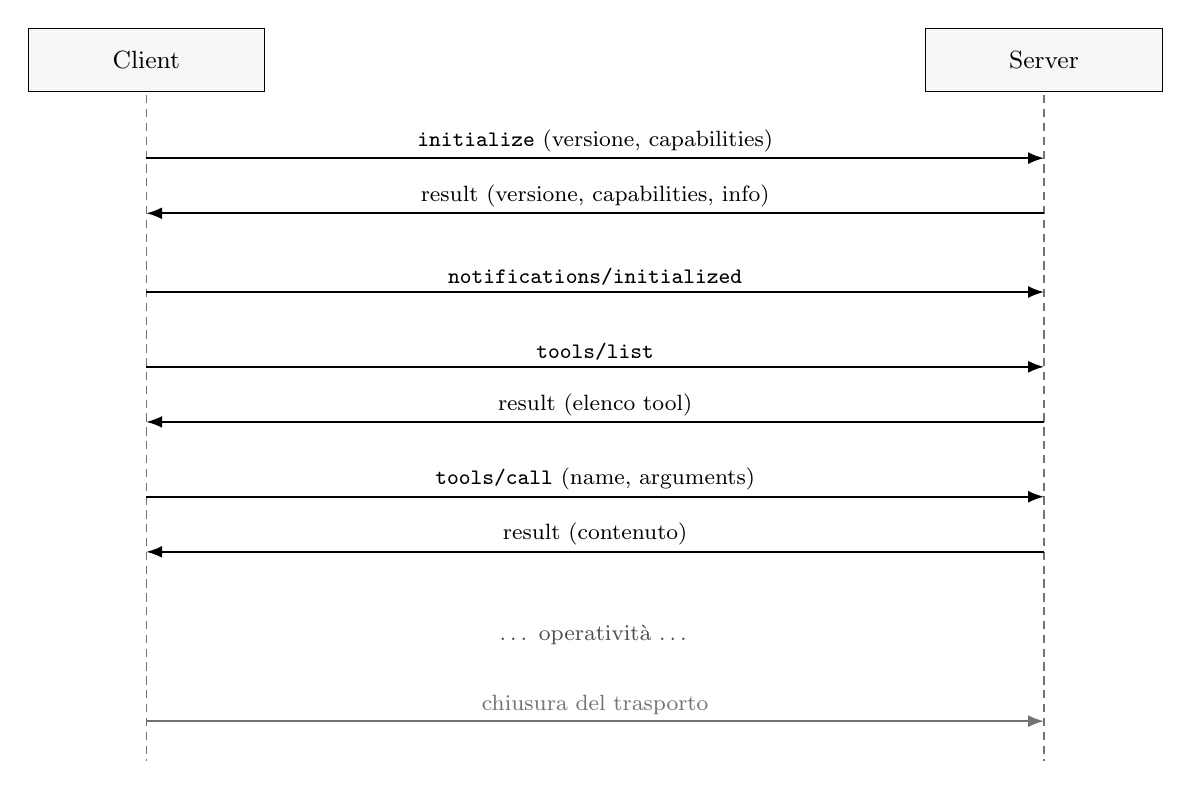
\begin{tikzpicture}[font=\small,
  head/.style={draw, minimum width=3.0cm, minimum height=8mm, align=center, fill=black!3},
  arr/.style={-{Latex[length=2mm,width=1.5mm]}, semithick},
  msg/.style={font=\footnotesize, inner sep=2pt}]

  \node[head] (c) at (0,0) {Client};
  \node[head] (s) at (11.4,0) {Server};
  \draw[densely dashed, black!55] (0,-0.45) -- (0,-8.9);
  \draw[densely dashed, black!55] (11.4,-0.45) -- (11.4,-8.9);

  \draw[arr] (0,-1.25) -- node[msg, above] {\texttt{initialize} (versione, capabilities)} (11.4,-1.25);
  \draw[arr] (11.4,-1.95) -- node[msg, above] {result (versione, capabilities, info)} (0,-1.95);
  \draw[arr] (0,-2.95) -- node[msg, above] {\texttt{notifications/initialized}} (11.4,-2.95);
  \draw[arr] (0,-3.9) -- node[msg, above] {\texttt{tools/list}} (11.4,-3.9);
  \draw[arr] (11.4,-4.6) -- node[msg, above] {result (elenco tool)} (0,-4.6);
  \draw[arr] (0,-5.55) -- node[msg, above] {\texttt{tools/call} (name, arguments)} (11.4,-5.55);
  \draw[arr] (11.4,-6.25) -- node[msg, above] {result (contenuto)} (0,-6.25);

  \node[font=\footnotesize, text=black!70] at (5.7,-7.3) {\dots\ operatività \dots};

  \draw[arr, black!55] (0,-8.4) -- node[msg, above] {chiusura del trasporto} (11.4,-8.4);
\end{tikzpicture}
\end{document}

